\subsubsection{Florida Tech} 

\paragraph*{Refurbishment of low-mass EIC Forward Tracker GEM detector prototype:}

The 3D-printed ABS pieces used in the original construction of the prototype chamber tended to deform and crack under tension causing the foils separated by a 1 mm gap to short out due to a lack of overall tension in the GEM stack. Consequently, we were not able to operate the prototype detector in the Fermilab beam test. We are replacing the ABS pieces with parts made from polyetheretherketone (PEEK), which is a polymer material with a tensile strength comparable to steel. Specifically, we are replacing the pull-outs that the GEM stack is tensioned against and two layers of inner frames. Fig.\ref{fig:installation} shows a test installation of the PEEK pull-outs in the detector.

\begin{figure}[h]
	\centering
	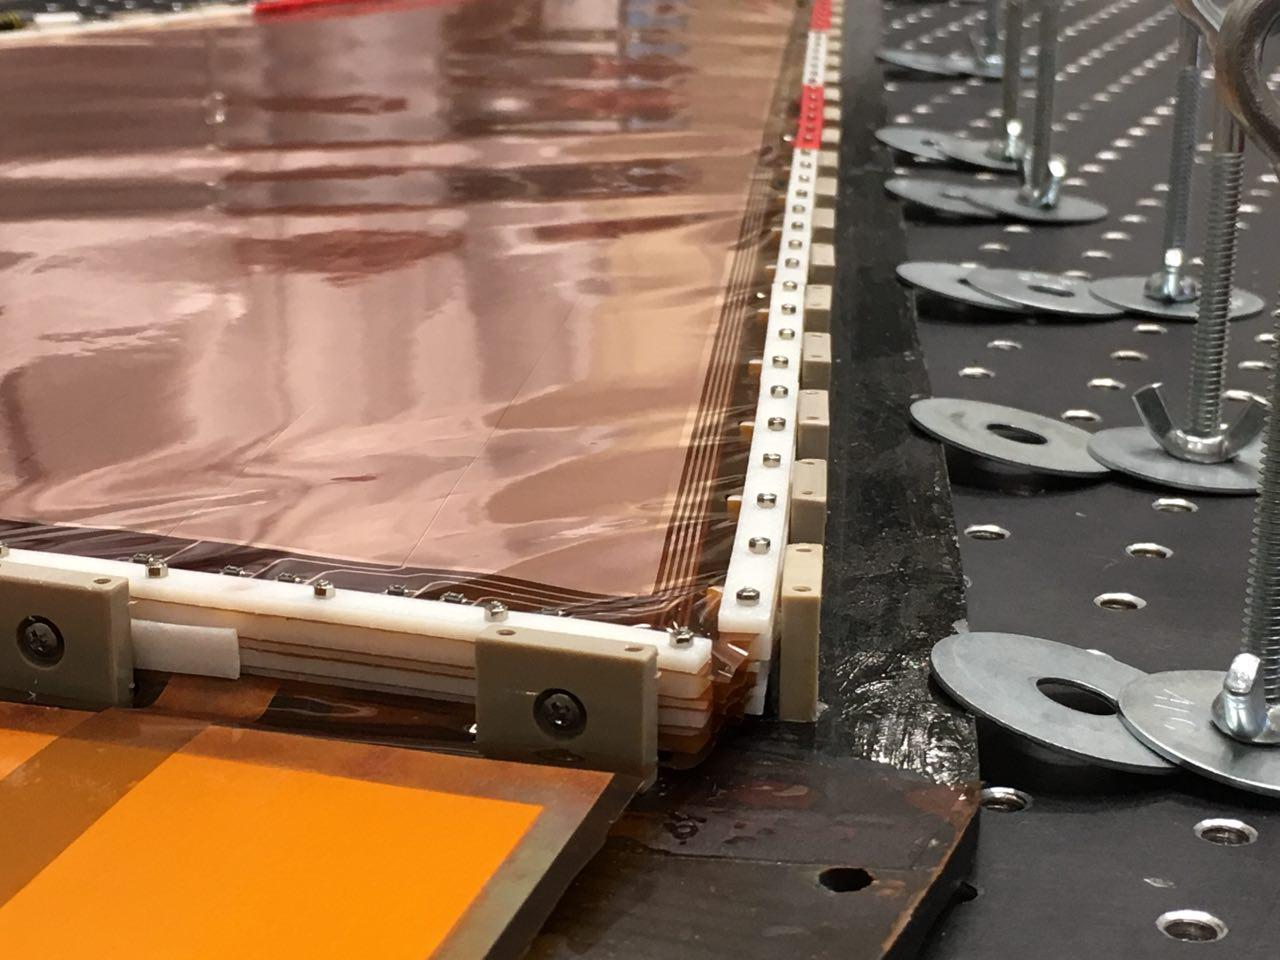
\includegraphics[width=0.9\textwidth]{FIT_plots/PEEK_Installation.jpg} 
	\caption{Test installation of PEEK pull-outs (gray blocks) in the low-mass GEM prototype.}
	\label{fig:installation}
\end{figure}

However, just as before we still observe shorts in the original GEM stack between those foils that are only 1 mm apart. To increase the spacing in the GEM stack, two new PEEK layers of inner frames with 2 mm thickness are being implemented. This will result in a stack with 3-2-2-2 mm gaps (drift, transfer 1, transfer 2, induction) instead of the previous 3-1-2-1 mm spacing. This replacement is possible due to the purely mechanical construction and stretching technique that we employ for the prototype.

For producing the pull-out parts, a 12"$\times$12" plate of 6 mm thick PEEK was machined on campus. In the original design of the inner frames, all pieces had the same short length of about 10 cm with 1 cm gaps between them. This resulted in warping of the GEM foils in the gaps. In the new design (Fig.\ref{fig:sidemid}), the side frames will be longer and fewer - more similar to the frame design of the CMS GE1/1 GEMs that this prototype is based on. The proper power setting of a laser cutter is currently being inverstigated for machining the inner frame pieces from a 12"$\times$6" plate of 2 mm thick PEEK, which is too thin for cutting on a NC machine. 

\begin{figure}[h]
	\centering
	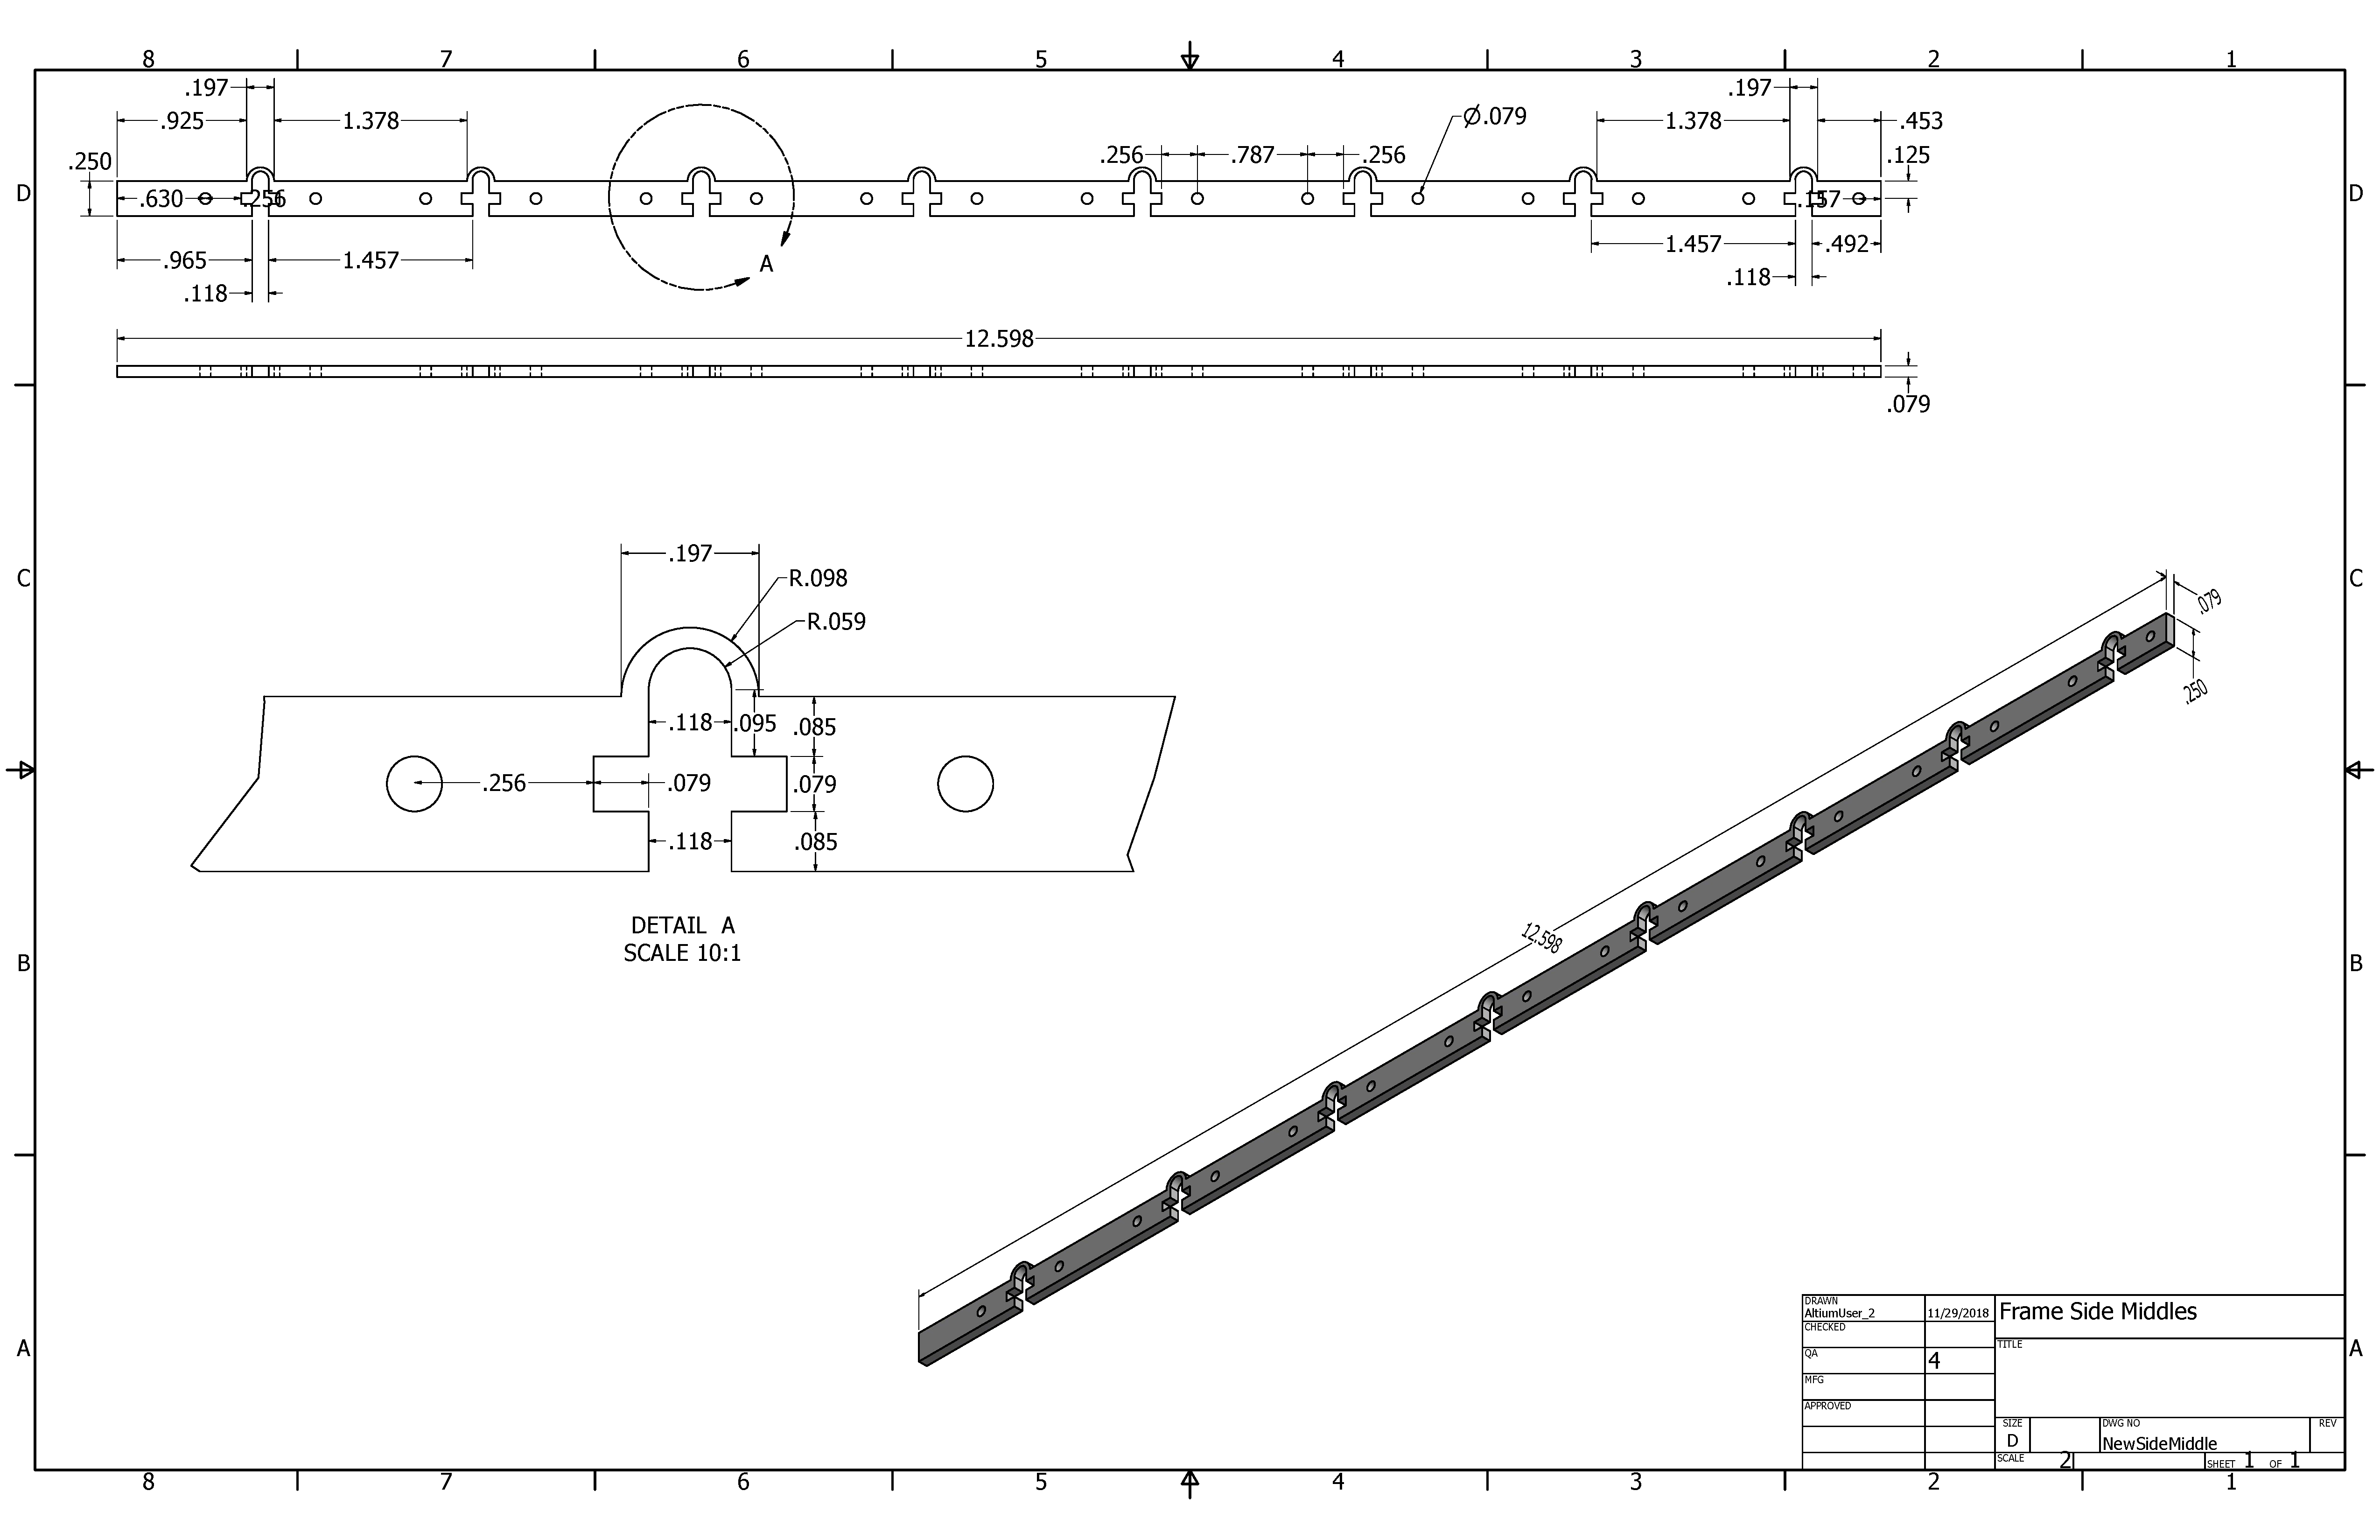
\includegraphics[width=0.9\textwidth]{FIT_plots/NewSideMiddle.pdf} 
	\caption{Design of longer middle sections of 2 mm side frames using PEEK.}
	\label{fig:sidemid}
\end{figure}



\paragraph*{R\&D on $\boldmath{\mu}$RWELL detector:} We have ordered a 10$\times$10 cm$^2$ resistive micro-well detector from CERN to begin some basic R\&D on this detector technology for fast tracking in the barrel region of the EIC detector. To complement the 2D readout with Cartesian strips chosen by the UVa group for their $\mu$RWELL detector prototype, we opted for a 1D zigzag strip readout foil based on the foil design that we had used for the 10$\times$10 cm$^2$ prototype\cite{Zhang:2017dqw} of the low-mass FT detector. We expect to receive this small detector in August or September 2018.



\paragraph*{EIC Simulations:} Undergraduate student Matt Bomberger continued his work on EIC simulations for investigating the impact that material budgets in the forward and backward regions will have on the overall EIC detector performance. He went to BNL in early August for a week to work directly with EicRoot expert Alexander Kiselev on the implementation of a forward tracker simulation based on Triple-GEMs. Working with a second undergraduate back at FIT, he succeeded in installing EicRoot in a Docker environment as well as directly in a CENTOS7 environment.

For a first study, he compared the momentum resolution of tracks measured with GEM chambers with standard copper foils vs.\ those with two chromium foils. A 3-1-2-1 mm GEM gap configuration and a beam of 1 GeV/c electrons emitted from the IP at 25$^\circ$ to the beamline are used. The geometry of this study and an example track are shown in Figure \ref{fig:geom}.

\begin{figure}[h]
	\centering
	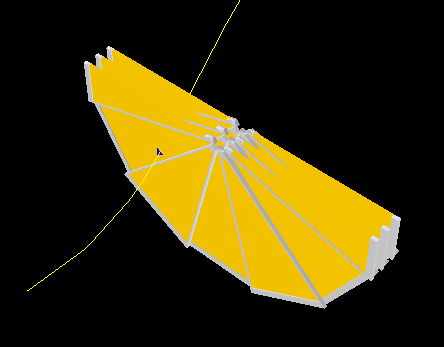
\includegraphics[width=0.9\textwidth]{FIT_plots/Geom_CrStdComp} % 
	\caption{EICroot simulation of a 1 GeV/c electron track reconstructed with 3 GEM rings in forward tracker region.}
	\label{fig:geom}
\end{figure}

The first configuration comprises all standard GEM foils, i.e.\ 5 $\mu$m thick planes of copper on both sides of a 50 $\mu$m thick plane of polyimide material. The distribution of the differences between reconstructed momentum and MC-truth momentum for this configuration has a Gaussian shape with a root mean square of 8.5\% (Figure \ref{fig:resolutions}(left)). For the configuration with chromium GEM foils, a 50 $\mu$ thick plane of polymide should be sandwiched between two planes of 200 nm thick planes of chromium. Since no direct method of using chromium foils is possible in EicRoot, the thickness of copper that would be equivalent to 2 foils with 200 nm of chromium and one of 5 $\mu$m of copper is plugged into the variable defining the thickness of copper in the GEM foils. In effect, this reduces the amount of copper basically by a factor three. The Gaussian plot of events versus momentum resolution for this chromium GEM configuration has an associated root mean square of 8.3\%. Comparing the RMS values for standard and chromium GEMs, one can see that they differ by only 0.2\% in favor of the chromium configuration. This implies that reducing the material from copper to chromium in two of the GEM foils has a minimal impact on the momentum resolution for this scenario. 

\begin{figure}[h]
	\centering
	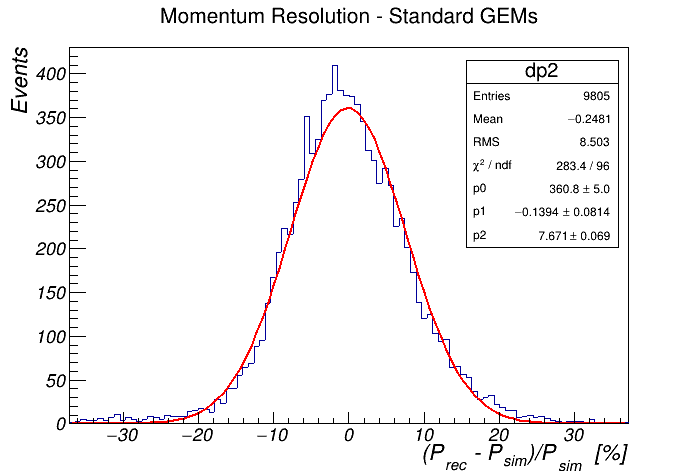
\includegraphics[width=0.49\textwidth]{FIT_plots/MomResStdGEM_25deg1GeV_101818}
	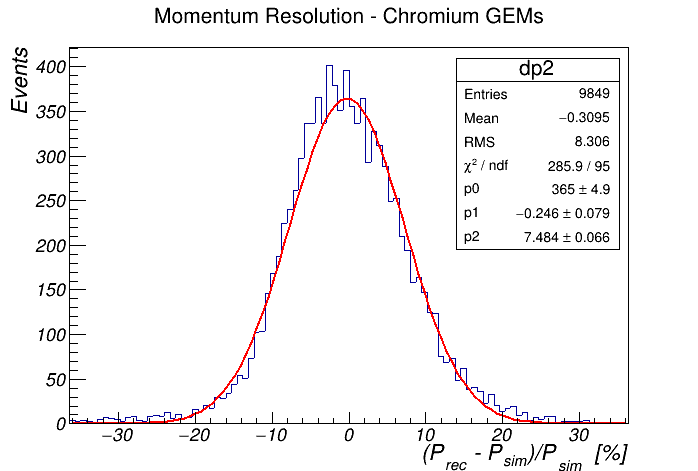
\includegraphics[width=0.49\textwidth]{FIT_plots/MomResCrGEM_25deg1GeV_101818} 
	\caption{Momentum resolutions for 1 GeV/c electron tracks measured with three rings of forward tracker GEMs in EICroot simulation (preliminary). Left: Standard GEMs with copper foils. Right: GEMs with two chromium foils and one copper foil.}
	\label{fig:resolutions}
\end{figure}



